\documentclass[pdflatex,a4paper,11pt,english]{scrreprt}
\usepackage[english]{varioref}
\usepackage[utf8]{inputenc}
\usepackage[T1]{fontenc}
\usepackage{listings}
\usepackage{graphicx}
\usepackage[svgnames]{xcolor}
\usepackage[pdfborder={0 0 0}]{hyperref}
\usepackage{url}
\usepackage{array}
\usepackage{textcomp}
\usepackage[english]{babel}

\clubpenalty = 10000
\widowpenalty = 10000
\displaywidowpenalty = 10000

\setcounter{secnumdepth}{3}
\setcounter{tocdepth}{4}

\begin{document}

\begin{titlepage}
\vspace*{4cm}
\begin{center}
\Large
Safety Critical Systems WS2008\\
Prof. Dr. Wagner\\
\vspace{4cm}
\normalsize
University of Applied Sciences Frankfurt\\
Faculty 2 - Computer Science and Engineering\\
M.Sc. - Program High-Integrity Systems\\
\vspace{2cm}
Insulin Pump Project\\
Documentation\\
Team 1\\
\vspace{2cm}
Wojciech Czylok, Rüdiger Gad, Elmar Köhler, Solomon Nega, Beril Olgun,\\
Nikolas Orlowski, Christina Paulsen, Jan Rabold, Murat Shahrashoub
\end{center}
\end{titlepage}

\tableofcontents

\listoffigures

%\lstlistoflistings

\chapter{Project Management}
\section{Organization}
\subsection{Development Process Model}
The spiral model is used for the main parts of our development.
See the project plan and the mind map for more detailt

\begin{figure}[htb]
\centering
\includegraphics[width=\textwidth]{images/Insulin_Pump_Mindmap.png}
\caption{
Mindmap of the problem
\label{fig:mindmap}
}
\end{figure}

\begin{figure}[htb]
\centering
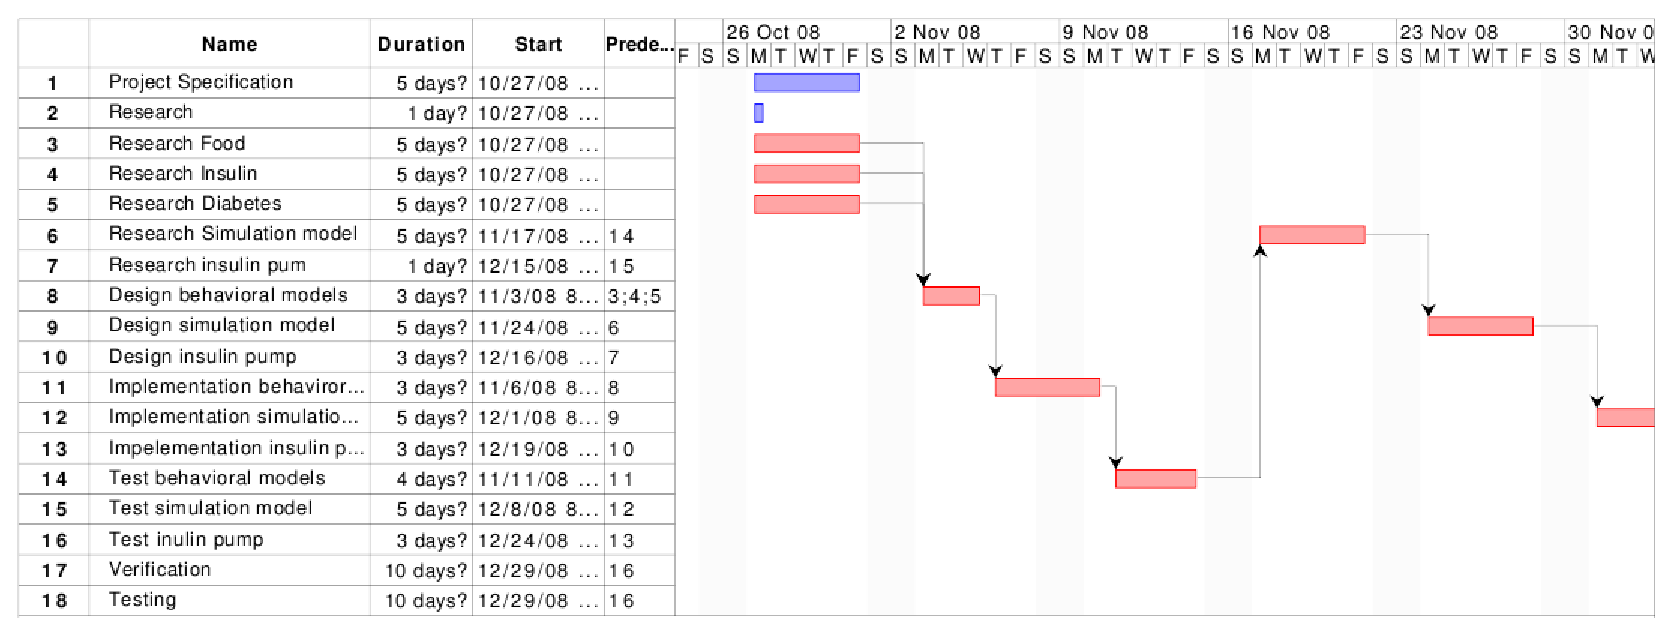
\includegraphics[width=\textwidth]{images/projectplan_page1}
\caption{
Project Plan Page 1
\label{fig:projectplan1}
}
\end{figure}

\begin{figure}[htb]
\centering
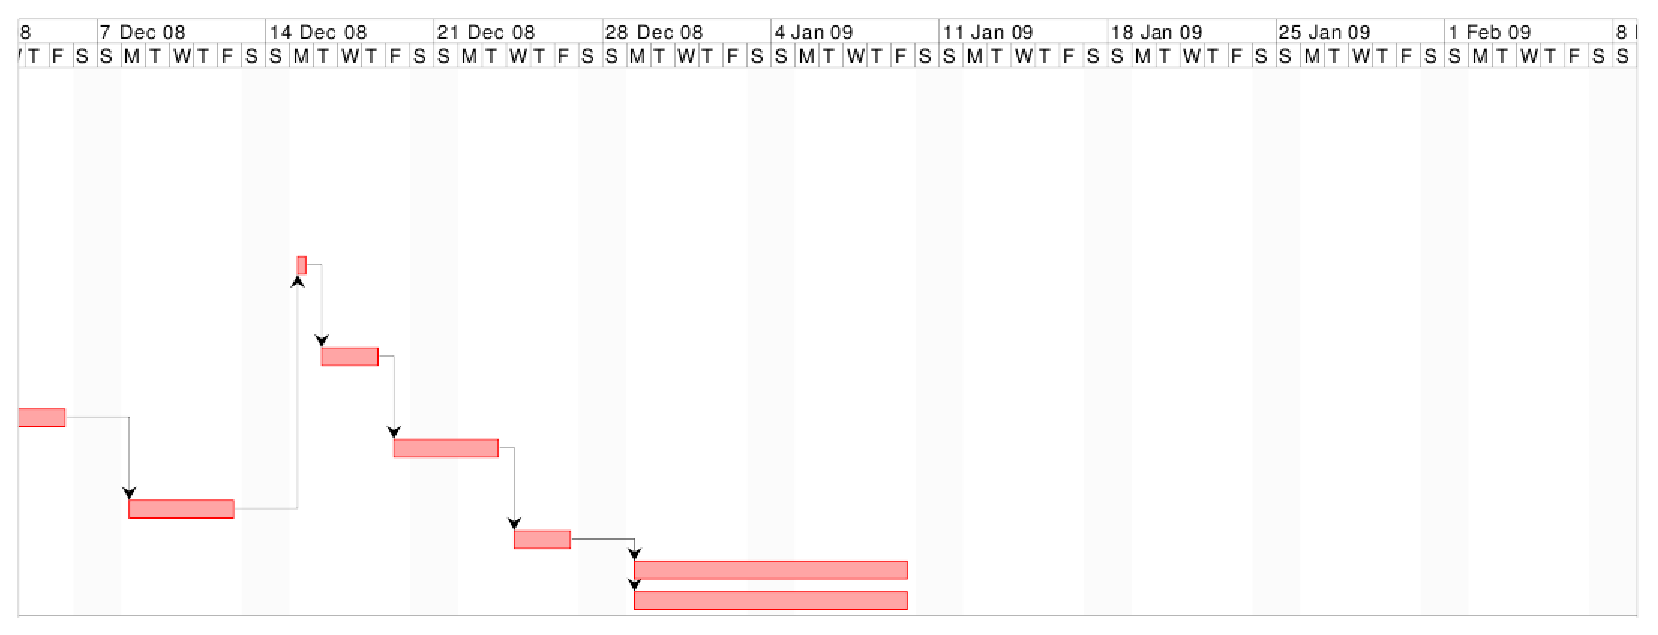
\includegraphics[width=\textwidth]{images/projectplan_page2}
\caption{
Project Plan Page 2
\label{fig:projectplan2}
}
\end{figure}
\newpage %TODO fix this hack

\subsection{Standardization}
Common value for measuring the blood glucose level is "mmol/l".
Programming language is Java.

\subsection{Specifications}
What do we want to achieve?
Simulation of the human body with diabetes and simulation of insulin pump.
Insulin pump has a sensor and automatic as well as manual injection.

\subsection{Risks}
People might get harmed or killed.
Project doesn't complete.

\subsubsection{Risk Handling}
Low glucose levels result in more serious effects on the health or even life then high levels.
So high glucose levels are prefered if there are situations when no clear preference can be made or one is in doubt.

\chapter{Development}
\section{Requirements Analysis}
Medical Problem, Theoretic background etc.

\subsection{Research at start / first iteration of spiral}
The research effort is split into three logical parts:
\begin{itemize}
  \item Diabetes
  \item Food
  \item Insulin
\end{itemize}
Details to the specific part of interest are explained in the following section.

\subsubsection{Diabetes}

\subsubsection{Food}
There are two major "indexes" which try to relate the type of food to the foods effect on the blood sugar level (glucose level).
The first such index is the so called "Glycemic Index" (GI) the second one the "Glycemic Load" (GL).
The GL tries to take some criteria according to the GI in account which have been widely critizized.
Still the GL and especially GI are both still being controversially discussed by experts.
Most of this discussion as it appears is mainly because people tend to use
diets based on these indexes in order to try to effect blood sugar level
without medicine. For a rating in a simplified simulation these indexes should
work out well, though the GL may be the one to prefer as it addresses some
weaknesses of the GI \cite{norden:glycemicindex}.

The time needed for food to affect the blood sugar can roughly be splitted up
into three groups of food which affect blood sugar level fast, moderate or
slowly \cite{mit:glycemicindex}.

\paragraph{Simulation}
In order to simulate the glucose level increase, after food has been eaten, programatically, mathematical models have to be made in order to calculate this process.
Here it is focused on the three main types of different foods with respect to speed of their absorbtion (i.e. how fast the gluscose level rises after a meal).
These three main types split up in

\begin{itemize}
  \item high glycemic (fast),
  \item moderate glycemic (intermediate) and
  \item low glycemic (slow) foods.
\end{itemize}

Unfortunately there are no mathematical models available for simulating this.
So in order to make a somewhat sane simulation there is the suggestion to use different formulas in order to simulate the different behavior of this foods.
The type of formula choosen should represent the behavior of glucose level absorbtion / increase in an approximate way.
The ammount of the glucose increase and roughly the timespan it occours in can be influenced by variables in these formulas.
Fortunately at least rough estimates can be made according to the absorbtion of
glucose in the blood as there exists a table which associates different foods
with theire behavior according to CI, CL etc. \cite{glycemicindex:table}.

\paragraph{Formulas}
So far two formulas have been evaluated.
Formula a (see figure \vref{fig:food_function_a}) has no skew and therefore is
symmetric. \begin{figure}[htb]
\centering
\includegraphics[width=\textwidth]{images/food_function_a}
\caption{Food Function A}
\label{fig:food_function_a}
\end{figure}
Formula b (see figure \vref{fig:food_function_b}) has a skew to the right. I.e.
it increases "slowly" two some point from which on it falls very abruptly. 
\begin{figure}[htb]
\centering
\includegraphics[width=\textwidth]{images/food_function_b}
\caption{Food Function B}
\label{fig:food_function_b}
\end{figure}
These formulas are attached with some sample data as Openoffice spread sheets under attachments.

\paragraph{Implementation}
In order to make it more flexible to choose different algorithms / formulas for
calculating the glucose values the Strategy pattern might be choosen. One
critical question with respect to the implementation is the choice of the used
data types for floatingpoint data as these data types are not guaranteed to be precise.

\subsubsection{Insulin}

\subsection{Research for second iteration of spiral / i.e. the body simulation}
General question:
How does insulin react with the glucose in the blood?
We need to know this in order to produce sane outputs.

\subsection{Requirements and Project Estimation}
The estimation of the project was done using COCOMO 2.
Therefore the metric used here is Lines Of Code (LOC).

First project estimation:
\begin{itemize}
  \item Behavior Simulation
  	\begin{itemize}
        \item eat (Guess: 450 LOC)
        \item insulin (Guess: 400 LOC)
        \item diabetes (Guess: 400 LOC)
    \end{itemize}
  \item Simulating Insulin Pump
  	\begin{itemize}
        \item actor (Insulin injection) (Guess: 600 LOC)
        \item sensor (Glucose Level Monitor) (Guess: 150 LOC)
        \item User Interface (Alarm/Input) (Guess: 500)
    \end{itemize}
\end{itemize} 
Guessed Estimation based on Experts Cocomo 2:
Effort 13.4 Person-months
Schedule 8.5 Months
\url{http://sunset.usc.edu/cgi-bin/expert_cocomo2000}

Second Project extimation:




\section{List of Requirements}
Requirement specification 
The overall goal of the project is to simulate
\begin{itemize}
  \item a) the human body with the illness diabetes and the aspects introduced
  by this illness. As well as the reaction on food and insulin injection.
  \item b) an insulin pump which reacts on the behavior of the the above given
  simulation of the human body with the illness diabetes.
\end{itemize}
The first step therefore is to provide a simulation of the human body with the
illness diabetes and the aspects food and insulin. 
Since this is quite a big task it is divided into modules. These modules should
first on their own simulate the behavior of diabetes, food and insulin and are
therefore called behavioral modules.

\subsection{Behavioral Modules}

\subsubsection{Diabetes Module}

\subsubsection{Food Module}
For reasons of simplification only the three major food groups are taken into
account.
These groups are 
\begin{itemize}
  \item high glycemic (fast),
  \item moderate glycemic (intermediate) and
  \item low glycemic (slow) foods.
\end{itemize}
In order to provide means to calculate the behavior of these groups
mathematical models need to be developed and / or researched to allow the
simulation.

\subsubsection{Insulin Module}
There are many insulin types, because of the given possibility to mix different 
insulin types together. Therefore we decided to implement the following three types of insulin:
\begin{itemize}
   \item Rapid-Acting
   \item Short-Acting
   \item Long-Acting
\end{itemize}
The different properties of each type are described in chapter 2.1.1.3!\\
DESCRIPTION OF THE MATHEMATICAL MODEL!\\

\subsection{Body Simulation}
The body simulation combines all behavioral modules and therefore simulates the
behavior of the human body with the illness diabetes.
Inputs of this body simulation are food and insulin.
Outputs are glucose and insulin values over time.

Concrete requirements are as follows:
\begin{itemize}
  \item Inputs must be realized as GUI and as inputs via given CSV-Files.
  \item Outputs must be realized as GUI and as CSV-Files.
  \item The behavioral modules created in the first step are combined to one
  large model.
\end{itemize} 

\subsection{Test Cases}
Test cases need to be designed for the complete simulation but as well for the
smaller parts (e.g. behavioral modules etc.).


\section{Analysis Model}


\section{Design Model}

\section{Code}

\end{document}
